\documentclass[a4paper,12pt]{extarticle}

%%%%%%%%%%%%
% Preamble

% The most important
\usepackage{examstylo}
%%% Provides the following:
%% For typesetting
% \mrm{} % shorthand mathrm
% \thus % Implication symbol
% \sm % small minus (for \sm2 - 2 = \sm 4)
% \meuro % neat euro sign
% \deg % degree
% \mli{} % multiletter identifier (prevents linebreak)
% \cldots % compact \ldots
% \oldots % orange compact \ldots (like in Kern)
% \rom{} % roman numeral
% \intextbullet % Make a bulletpoint
% \lognl[base] % make a logarithm base base
% \deriv{y}{x} % make total derivative dy/dx
%
%% For control
% \comment{} % comment everything inside
% \insertemptypage % Insert an empty page
% \begin{multicols}{2} <subquestions here> \end{multicols} % For two-column subquestions
%
%% And some colors
% \red{}
% \blue{}
% \orange{} % Like in Kern

%%% Some notes:
% \newsubquestion{}{} works with package paracol to make two columns. if you want a newline after the subquestion, put the \newline INSIDE the question txt (i.e., {example text\newline}) 
% use \begin{multicols}{2} for two-column subquestions. its not perfect but so arent you
  % It will force an empty line above (and below?) use \vspace{-\lineheight} to remedy
% Watch out with a \footnote: margin notes do not move with the text to the newpage after a footnote was inserted.
% You can use \insertemptypage to insert an empty page




%%%%% %%%%% Options!
%% Uncomment this to use points from Questions (ignored if use points from subquestions)
\UsePointsFromQuestions % < This
%% Uncomment this to use points from SUBquestions
%\UsePointsFromSubQuestions % < This
%% Uncomment this to make a full title page
\MakeTheFullTitlePage % < This
%% Uncomment this to make a simple title on the first page (ignored if make full titlepage)
%\MakeTheSimpleTitlePage % < This
%% Uncomment this to make the formula page
\MakeTheFormulaPage % < This
%% Uncomment this to make the worksheets
\MakeTheWorksheetPages % < This

%% Uncomment this to use Arial (Ugly!)
\UseArialFont % < This


%% Footer options
\SetFooterOptions[% Set options for the footer
  showleft=True,%=True
  showcenter=True,%=True
  showright=True,%=True
  ]{}

%% Exercise options
\SetExerciseOptions[% Set options for exercises
  PutExerciseOnNewPage=True,%=True to show every (except first) exercise on a new page
  PutFirstExerciseOnNewPage=True,%=True to have the first exercise on a new page
  firstexercisevskip=\baselineskip,%=\baselineskip if first exercise not on new page, how much vspace before?
  ExerciseResetQuestionCount=False,%=False, at new exercise, reset the question counter?
  ]{}

%% Worksheet options
\SetWorksheetOptions[% Set options for exercises
  ShowTitle=True,%=True to show the title on the first page of the worksheets
  ]{}
  
%% Simple titlepage options
\SetSimpleTitleOptions[% Set options for exercises
  thestyle=Default,%=Default [Attempts to look like full titlepage, but small], =Exerciselike [Looks more like the exercise seperator]
  ]{}
  
%%%%% %%%%% BEGIN document
\begin{document}

%%%%% Title Page Settings
\title{Test for a test}
\extratitletext{{\Large Versie A}} % extra concise info e.g, {\Large Versie A}
\leftfoottext{testtest-v0} % Text in the left box of the footer

\date{Zondag 09-02-1992}
\time{09:02\enspace--\enspace16:20\,uur}

\noteforthelastpage{% Put text here to have a note on the last page
%\textbf{Credit:} Hello this is credit which is shown on the last page.
} % end text for lastpage note

%%% Put text for the title page Here
% Use \totqstns and \totpts to reference total questions and total points resp.
\titlepagetext{
Bij dit examen hoort een uitwerkbijlage. 

\vfill
Dit examen bestaat uit \totqstns\ vragen.\par
Voor dit examen zijn maximaal \totpts\ punten te behalen.\par
Voor elk vraagnummer staat hoeveel punten met een goed antwoord behaald
kunnen worden.\\

Als bij een vraag een verklaring, uitleg of berekening vereist is, worden aan het antwoord meestal geen punten toegekend als deze verklaring, uitleg of berekening ontbreekt.\\
 
Geef niet meer antwoorden (redenen, voorbeelden e.d.) dan er worden gevraagd. Als er bijvoorbeeld twee redenen worden gevraagd en je geeft meer dan twee redenen, dan worden alleen de eerste twee in de beoordeling meegeteld.
} % End of the title page text

%%% Put text here for the simple title on the first page
% Use \totqstns and \totpts to reference total questions and total points resp.
\simpletitletext{
\textit{Dit examen bestaat uit \totqstns\ vragen, waarvoor maximaal \totpts\ punten zijn te behalen.\\
Veel succes en plezier!\\
  }
}


% Make title pages if instructed to
\ifmakefulltitlepage
  \maketitlepage % inserts a \newpage
\else
  \ifmakesimpletitlepage
    \makesimpletitleonfirstpage % does not insert a \newpage
  \fi
\fi


\pagestyle{mainpagestyle} % Apply the main style
%%%%% Formula Page (?)

\formulapagetext{% Put text here for the formula page(s)

\textbf{Differenti\"eren}\\[0.5\baselineskip]\noindent
\begin{tabular}{lll}
\hline\hline
Naam van de regel & Functie & Afgeleide \\\hline
somregel & $s(x) = f(x)+g(x)$ & $s'(x) = f'(x) + g'(x)$ \\
verschilregel & $v(x) = f(x)-g(x)$ & $v'(x) = f'(x) - g'(x)$ \\
productregel & $p(x) = f(x)\cdot g(x)$ & $p'(x) = f'(x)\cdot g(x) + f(x)\cdot g'(x)$ \\
quoti\"entregel & $q(x) = \frac{f(x)}{g(x)}$ & $q'(x) = \frac{f'(x)\cdot g(x) - f(x)\cdot g'(x)}{(g(x))^2}$ \\
kettingregel & $k(x) = f(g(x))$ & $k'(x) = f'(g(x))\cdot g'(x)$ of  $\deriv{k}{x} = \deriv{f}{g}\cdot\deriv{g}{x}$ \\
\hline
\end{tabular}


} % End of formula page text

% Make the formula page if instructed to
\ifmaketheformulapage
  \makeformulapage
\fi

%%%%% Begin With the Body
\makeatletter\ifOptExc@firstexconnewpage
  \setmainpagegeometry
\fi\makeatother

%%% New exercise
\newexercise{Lorem} \label{exc:lorem}

%\begin{wrapfigure}[]{r}{0.3\textwidth} % Use for illustrations, not figures
%\begin{wrapfigure}[<number of lines>]{<capital for float>}{0.5\textwidth}
%\centering
%    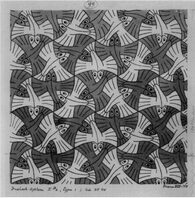
\includegraphics[width=0.25\textwidth]{escher.jpg}
% \caption{}
%\end{wrapfigure}

Lorem ipsum dolor sit amet, consectetur adipiscing elit, sed do eiusmod tempor incididunt ut labore et dolore magna aliqua. Ut enim ad minim veniam, quis nostrud exercitation ullamco laboris nisi ut aliquip ex ea commodo consequat.
Duis aute irure dolor in reprehenderit in voluptate velit esse cillum dolore eu fugiat nulla pariatur. $\lognl[4] 4 + \lognl(5x+3)$

Excepteur sint occaecat cupidatat non proident, sunt in culpa qui officia deserunt mollit anim id est laborum. Welkom bij vraag \nameref{exc:lorem}.\newline

\newquestion[2]{quis nostrud exercitation ullamco laboris nisi ut aliquip ex ea commodo consequat.} \label{q:vraag}

Lorem ipsum dolor sit amet, consectetur adipiscing elit, sed do eiusmod tempor incididunt ut labore et dolore magna aliqua. Ut enim ad minim veniam, quis nostrud exercitation ullamco laboris nisi ut aliquip ex ea commodo consequat.\\

\makefigure{width=0.6\textwidth}{random_graph.png}{Optional caption} % {<kwargs for includegraphics>}{<figpath>}{<caption, leave empty for no caption>}

Duis aute irure dolor in reprehenderit in voluptate velit esse cillum dolore eu fugiat nulla pariatur. Excepteur sint occaecat cupidatat non proident, sunt in culpa qui officia deserunt mollit anim id est laborum.

\newquestion[2]{quis nostrud exercitation ullamco laboris nisi ut aliquip ex ea commodo consequat.} \label{q:vraagvb}
\begin{itemize}
    \item item 1
    \item item 1
\end{itemize}
Lorem ipsum dolor sit amet, consectetur adipiscing elit, sed do eiusmod tempor incididunt ut labore et dolore magna aliqua. Ut enim ad minim veniam, quis nostrud exercitation ullamco laboris nisi ut aliquip ex ea commodo consequat. 

Duis aute irure dolor in reprehenderit in voluptate velit esse cillum dolore eu fugiat nulla pariatur.\newline

Lorem ipsum dolor sit amet, consectetur adipiscing elit, sed do eiusmod tempor incididunt ut labore et dolore magna aliqua. Ut enim ad minim veniam, quis nostrud exercitation ullamco laboris nisi ut aliquip ex ea commodo consequat. 

Yo vivía tan distinto, algo hermoso
Algo divino, lleno de felicidad
Yo sabia de alegrías, la belleza de la vida
Pero no de soledad, pero no de soledad
De eso y muchas cosas más
Yo jamás sufrí, yo jamás lloré
Yo era muy feliz, yo vivía muy bien

\insertemptypage % EMPTY PAGE

\newquestion[2]{\label{q:vraagvbb}quis nostrud exercitation ullamco laboris nisi ut aliquip ex ea commodo consequat.\newline}

\newquestion[3]{\label{q:vraagvbbb}quis nostrud exercitation ullamco laboris nisi ut aliquip ex ea commodo consequat.\newline} 

\newquestion[3]{\label{q:vraagvbbbb}quis nostrud exercitation ullamco laboris nisi ut aliquip ex ea commodo consequat. ea commodo consequat.} 
\newsubquestion[2]{No sabía, de tristezas, ni de lágrimas, Ni nada, que me hicieran llorar,}
\newsubquestion[2]{Yo sabía de cariño, de ternura. Porque a mí desde pequeño Eso me enseño mamá,}
\newsubquestion[2]{eso me enseño mamá Eso y muchas cosas más.\label{sq:ex}}
\newsubquestion[2]{Yo jamás sufrí, yo jamás lloré. Yo era muy feliz, yo vivía muy bien\newline}

Lorem ipsum dolor sit amet, consectetur adipiscing elit, sed do eiusmod tempor incididunt ut labore et dolore magna aliqua. Ut enim ad minim veniam, quis nostrud exercitation ullamco laboris nisi ut aliquip ex ea commodo consequat. 

\newquestion[1]{quis nostrud exercitation ullamco laboris nisi ut aliquip ex ea commodo consequat.}\label{q:vraagvbbbbb}%
\newsubquestion[2]{No sabía, de tristezas, ni de lágrimas, Ni nada, que me hicieran llorar,}

\newsubquestion[2]{Yo sabía de cariño, de ternura. Porque a mí desde pequeño Eso me enseño mamá,}

\newsubquestion[2]{eso me enseño mamá Eso y muchas cosas más.}

Lorem ipsum dolor sit amet, consectetur adipiscing elit, sed do eiusmod tempor incididunt ut labore et dolore magna aliqua. Ut enim ad minim veniam, quis nostrud exercitation ullamco laboris nisi ut aliquip ex ea commodo consequat. 

\newsubquestion[2]{Yo jamás sufrí, yo jamás lloré. Yo era muy feliz, yo vivía muy bien\newline}

\newquestion[3]{quis nostrud exercitation ullamco laboris nisi ut aliquip ex ea commodo consequat.} \label{q:vraagvbvbvb}


%%% New exercise
\newexercise{Lorem 2} \label{exc:second}

In exercise \ref{exc:lorem} and \ref{exc:second}, question~\ref{q:vraag} or question~\ref{q:vraagvb}. Also subquestion~\ref{q:vraagvbvb}\ref{sq:example} and~\ref{q:vraagvbbbb}\ref{sq:ex}.

Lorem ipsum dolor sit amet, consectetur adipiscing elit, sed do eiusmod tempor incididunt ut labore et dolore magna aliqua. Ut enim ad minim veniam, quis nostrud exercitation ullamco laboris nisi ut aliquip ex ea commodo consequat. 
\begin{itemize}
    \item item 1
    \item item 1
\end{itemize}
Duis aute irure dolor in reprehenderit in voluptate velit esse cillum dolore eu fugiat nulla pariatur. 

\newquestion[2]{\label{q:vraagdrie}question question question\newline}  

Excepteur sint occaecat cupidatat non proident\footnote{Nou ja zeg een footnote}, sunt in culpa qui officia deserunt mollit anim id est laborum. In equation~\ref{eq:equation} and~\ref{eq:equationtwo}.

\begin{equation} \label{eq:equation}
    K=3x^2 - 3 = 0 
\end{equation}

\begin{itemize}
    \item $K$ de koek
    \item item 1
\end{itemize}
Lorem ipsum dolor sit amet, consectetur adipiscing elit, sed do eiusmod tempor incididunt ut labore et dolore magna aliqua. Ut enim ad minim veniam, quis nostrud exercitation ullamco laboris nisi ut aliquip ex ea commodo consequat.\\

\begin{equation} \label{eq:equationtwo}
    x^2 - 3 = 0
\end{equation}

\newquestion[2]{\label{q:vraagvier}question question question\newline}

Duis aute irure dolor in reprehenderit in voluptate velit esse cillum dolore eu fugiat nulla pariatur.

\newquestion[2]{\label{q:vraagvijf}question question question\newline}  

\newquestion[2]{question question question question question question question question question question question question question question question question question question question question question\newline}  \label{q:vraagzes}

\newpage
Excepteur sint occaecat cupidatat non proident, sunt in culpa qui officia deserunt mollit anim id est laborum.


\newquestion[3]{\label{q:vraagvbvb} quis nostrud exercitation ullamco laboris nisi ut aliquip ex ea commodo consequat. ea commodo consequat.}\vspace{-\lineheight}%\vspace{-0.83333\baselineskip}  
\begin{multicols}{2}%
\newsubquestion[2]{$y=x^2-3$ \label{sq:example}}
\newsubquestion[2]{$L=4\pi R^2 \sigma T^4$}
\newsubquestion[2]{\label{sq:subq}Yo jamás sufrí, yo jamás lloré. Yo era muy feliz, yo vivía muy bien}
\columnbreak% Notice the columnbreak
\newsubquestion[2]{$y=x^2-3$}
\newsubquestion[2]{$y=x^2-3$}
\newsubquestion[2]{$y=x^2-3$}
\end{multicols}
Excepteur sint occaecat cupidatat non proident, sunt in culpa qui officia deserunt mollit anim id est laborum.





%%% This is the end (do not touch)
\lastpageofthetest\
%%

%%%%% HERE STARTS THE WORKSHEETS
\worksheetcontent{% Put content here for the worksheets
                  % Use \refquestion{<label>} to refer to a question
\refquestion{q:vraag}\newline
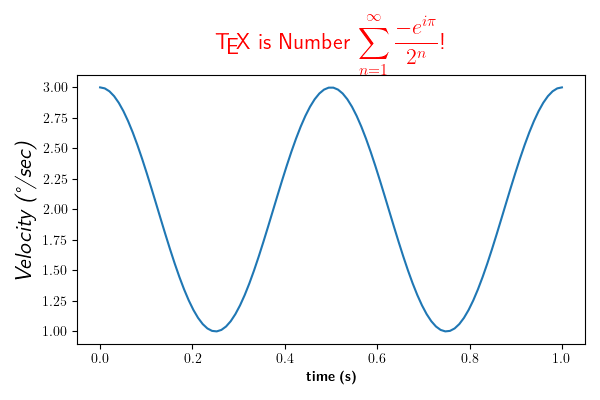
\includegraphics[width=0.8\textwidth]{random_graph.png}

\vfill

\refquestion{q:vraagvier} (\nameref{q:vraagvier})\newline
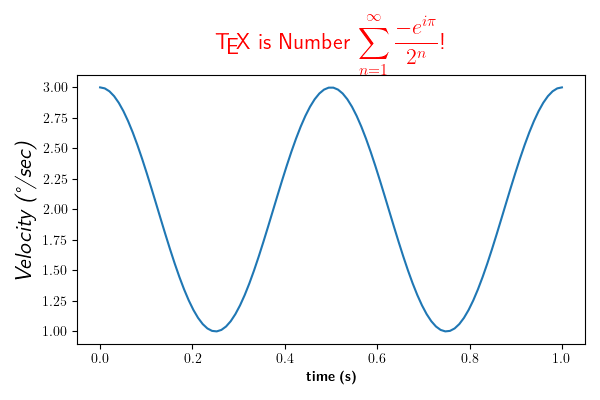
\includegraphics[width=0.8\textwidth]{random_graph.png}

\newpage

\refquestion{q:vraagvijf} en \refquestion{q:vraagzes}\newline
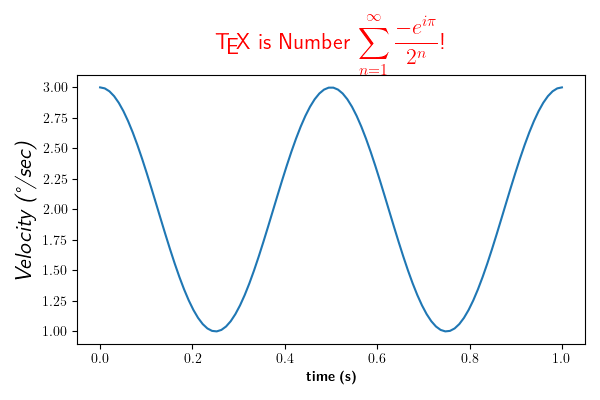
\includegraphics[angle=90,width=0.8\textwidth]{random_graph.png} % Sidenote: The rotating package introduces a sidewaysfigure

} % End worksheet content

% Make the worksheet pages if instructed to
\ifmakeworksheetpages
  \makeworksheets
\fi



\end{document}
